\documentclass[aspectratio=169]{beamer}

% Shared Beamer settings for Applied Machine Learning lectures (UPES).
% Keep this file free of \documentclass to allow reuse via \input.

% Allow lecture sources to use shared theme/assets without copying them into each lecture folder.
% NOTE: These paths are relative to `Unit-xx/Lecture-yy/latex/` (and `Lab/Experiment-xx/latex/`).
\makeatletter
\def\input@path{{../../../_shared/}{../../../_shared/UPES-Beamer-Theme/}}
\makeatother

\usetheme{UPES}
\setbeamertemplate{navigation symbols}{}

\usepackage{amsmath}
\usepackage{amssymb}
\usepackage{booktabs}
\usepackage{graphicx}
\usepackage{hyperref}
\usepackage{xcolor}
\usepackage{listings}

% Code listings (Python-oriented for this subject).
\lstset{
  language=Python,
  basicstyle=\ttfamily\small,
  keywordstyle=\color{blue},
  commentstyle=\color{gray},
  stringstyle=\color{teal},
  showstringspaces=false,
  columns=fullflexible,
  breaklines=true
}

\usepackage{tikz}
\usetikzlibrary{arrows.meta,positioning,shapes.geometric,calc,fit,backgrounds}

% Per-slide source line (references shown on the slide itself).
\newcommand{\slidesources}[1]{%
  \vfill
  {\tiny\color{gray}\raggedright\sloppy\parbox{\linewidth}{Sources: #1}\par}%
}

% Unit-wise source strings for this subject (used by slides/notes).
% Path is relative to the lecture `latex/` folder (the compilation CWD).
% Source strings for Applied Machine Learning (CSAI2017P) — used by slides + notes.
% Prescribed texts and reference books are taken from the course syllabus.
% Support texts are the author-hosted open-access editions:
%   statlearning.com            (ISL with Python)
%   probml.github.io/pml-book   (Murphy, Probabilistic Machine Learning)
%   d2l.ai                      (Dive into Deep Learning)
%   mml-book.github.io          (Mathematics for Machine Learning)

\newcommand{\AMLRepoURL}{https://github.com/tali7c/Applied-Machine-Learning}

% --- prescribed -------------------------------------------------------------
\newcommand{\AMLPrescribed}{%
M\"uller and Guido, \textit{Introduction to Machine Learning with Python}, O'Reilly, 2016.;%
Bishop, \textit{Pattern Recognition and Machine Learning}, Springer, 2006.;%
Murphy, \textit{Machine Learning: A Probabilistic Perspective}, MIT Press, 2012.;%
Han, Kamber and Pei, \textit{Data Mining: Concepts and Techniques} (3e), Morgan Kaufmann, 2012.%
}

% --- unit-wise ---------------------------------------------------------------
\newcommand{\AMLUnitISources}{%
M\"uller and Guido, \textit{Introduction to Machine Learning with Python}, Ch. 1.;%
Bishop, \textit{Pattern Recognition and Machine Learning}, Ch. 1.;%
Murphy, \textit{Probabilistic Machine Learning: An Introduction}, MIT Press, 2022, Ch. 1.;%
Mitchell, \textit{Machine Learning}, McGraw Hill, 1997, Ch. 1.;%
Scikit-learn documentation, accessed 2026-08-04.%
}

\newcommand{\AMLUnitIISources}{%
Bishop, \textit{Pattern Recognition and Machine Learning}, \S1.5, \S4.3, \S7.1.;%
Zhang, Lipton, Li and Smola, \textit{Dive into Deep Learning}, \S3.4.;%
Shalev-Shwartz and Ben-David, \textit{Understanding Machine Learning}, Ch. 15.;%
Murphy, \textit{Probabilistic Machine Learning: An Introduction}, Ch. 5.%
}

\newcommand{\AMLUnitIIISources}{%
Zhang, Lipton, Li and Smola, \textit{Dive into Deep Learning}, Ch. 12 (Optimization Algorithms).;%
Deisenroth, Faisal and Ong, \textit{Mathematics for Machine Learning}, Ch. 7.;%
Kingma and Ba, ``Adam: A Method for Stochastic Optimization,'' ICLR 2015.;%
Ruder, ``An overview of gradient descent optimization algorithms,'' arXiv:1609.04747, 2016.%
}

\newcommand{\AMLUnitIVSources}{%
Han, Kamber and Pei, \textit{Data Mining: Concepts and Techniques} (3e), Ch. 3.;%
M\"uller and Guido, \textit{Introduction to Machine Learning with Python}, Ch. 3--4.;%
James, Witten, Hastie, Tibshirani and Taylor, \textit{An Introduction to Statistical Learning with Python}, Ch. 5--6, 12.;%
Scikit-learn documentation (preprocessing, model selection), accessed 2026-08-04.%
}

\newcommand{\AMLUnitVSources}{%
James et al., \textit{An Introduction to Statistical Learning with Python}, Ch. 3--6.;%
Bishop, \textit{Pattern Recognition and Machine Learning}, Ch. 3.;%
Deisenroth, Faisal and Ong, \textit{Mathematics for Machine Learning}, Ch. 9.;%
M\"uller and Guido, \textit{Introduction to Machine Learning with Python}, \S2.3.%
}

\newcommand{\AMLUnitVISources}{%
Han, Kamber and Pei, \textit{Data Mining: Concepts and Techniques} (3e), Ch. 8--9.;%
James et al., \textit{An Introduction to Statistical Learning with Python}, Ch. 8--9.;%
Bishop, \textit{Pattern Recognition and Machine Learning}, Ch. 4--5, 7, 14.;%
Zhang et al., \textit{Dive into Deep Learning}, Ch. 5.%
}

\newcommand{\AMLUnitVIISources}{%
Han, Kamber and Pei, \textit{Data Mining: Concepts and Techniques} (3e), Ch. 10.;%
James et al., \textit{An Introduction to Statistical Learning with Python}, Ch. 12.;%
M\"uller and Guido, \textit{Introduction to Machine Learning with Python}, \S3.5.;%
Ester, Kriegel, Sander and Xu, ``A density-based algorithm for discovering clusters (DBSCAN),'' KDD 1996.%
}

\newcommand{\AMLLabSources}{%
M\"uller and Guido, \textit{Introduction to Machine Learning with Python}, companion notebooks.;%
McKinney, \textit{Python for Data Analysis} (3e), O'Reilly, 2022.;%
Scikit-learn user guide, accessed 2026-08-04.;%
Matplotlib and Seaborn documentation, accessed 2026-08-04.%
}



\graphicspath{{../figures/}{../images/}{../../../_shared/}{../../../_shared/UPES-Beamer-Theme/}}

\title[Applied Machine Learning]{Applied Machine Learning}
\subtitle{Unit 06 -- Lecture 15: Bayesian Algorithms}
\author{Tofik Ali}
\institute{School of Computer Science, UPES Dehradun}
\date{Autumn 2026}

% ---- a compact "output" block so code and its result sit together ----------
\lstdefinestyle{outblk}{
  basicstyle=\ttfamily\scriptsize\color{black!75},
  backgroundcolor=\color{black!5}, frame=leftline, framerule=2pt,
  rulecolor=\color{black!30}, breaklines=true, columns=fullflexible,
  keepspaces=true,   % several outputs below are aligned tables
  language={},       % printed output is not Python: do not syntax-highlight it
  xleftmargin=4pt, aboveskip=1pt, belowskip=1pt, literate={-}{{-}}1}
\lstnewenvironment{outblk}{\lstset{style=outblk}}{}

\begin{document}

\UPESCoverFrame
\setcounter{framenumber}{0}

\begin{frame}
  \titlepage
  \begin{center}
    \footnotesize The classifier you can derive from one line of probability
    theory\\[0.25em]
    \footnotesize Topic focus: \textbf{a $99\%$ accurate test, and a
    $16.67\%$ answer}\\[0.25em]
    \footnotesize Repository: \texttt{\AMLRepoURL}
  \end{center}
  \slidesources{\AMLUnitVISources}
\end{frame}

\begin{frame}{Quick Links}
  \centering
  \hyperlink{sec:bayes}{\beamerbutton{Bayes' theorem}}\hspace{0.4em}
  \hyperlink{sec:decide}{\beamerbutton{MAP and ML}}\hspace{0.4em}
  \hyperlink{sec:naive}{\beamerbutton{The naive assumption}}\hspace{0.4em}
  \hyperlink{sec:hand}{\beamerbutton{By hand}}\hspace{0.4em}
  \hyperlink{sec:zero}{\beamerbutton{Zero frequency}}\hspace{0.4em}
  \hyperlink{sec:logs}{\beamerbutton{Logs}}\hspace{0.4em}
  \hyperlink{sec:gauss}{\beamerbutton{Gaussian NB}}\hspace{0.4em}
  \hyperlink{sec:calib}{\beamerbutton{Bad probabilities}}\hspace{0.4em}
  \hyperlink{sec:hurts}{\beamerbutton{Where it hurts}}\hspace{0.4em}
  \hyperlink{sec:summary}{\beamerbutton{Summary}}
\end{frame}

\begin{frame}{Agenda}
  \tableofcontents
\end{frame}

\begin{frame}[shrink=6]{How this lecture works}
  \begin{columns}[T]
    \begin{column}{0.48\textwidth}
      \begin{block}{Every idea appears twice}
        \begin{enumerate}
          \item \textbf{By hand} --- one test result, fourteen weather
            records, four words in an e-mail, one petal width. Small enough
            to check on paper, and small enough to appear in a test.
          \item \textbf{In code} --- the same arithmetic through
            \texttt{CategoricalNB}, \texttt{MultinomialNB} and
            \texttt{GaussianNB}, agreeing to eleven decimal places.
        \end{enumerate}
      \end{block}
    \end{column}
    \begin{column}{0.48\textwidth}
      \begin{alertblock}{Commit before you look}
        Five slides ask you to write a number down before it is revealed.
        \textbf{The first one is the whole lecture.} Almost everybody gets it
        wrong, and being wrong on paper is how the idea sticks.
      \end{alertblock}
    \end{column}
  \end{columns}
  \vspace{0.4em}
  \begin{center}
    \small Two numbers to carry out: a positive result on a $99\%$-sensitive
    test means \textbf{a $16.67\%$ chance of disease}; and a product of
    $148$ probabilities is, in \texttt{float64}, \textbf{exactly $0.0$}.
  \end{center}
\end{frame}

\begin{frame}[shrink=6]{Four datasets, one seed --- and one thing a seed cannot fix}
  \begin{columns}[T]
    \begin{column}{0.48\textwidth}
      \begin{block}{The data}
        \small scikit-learn's bundled \texttt{load\_iris},
        \texttt{load\_wine}, \texttt{load\_breast\_cancer} and
        \texttt{load\_digits}; a twelve-message spam corpus typed out in the
        source; synthetic documents drawn from the seed. Nothing is
        downloaded.
      \end{block}
    \end{column}
    \begin{column}{0.48\textwidth}
      \begin{block}{The randomness}
        \small One seed: \texttt{np.random.default\_rng(0)} and
        \texttt{random\_state=0}. Every listing that draws or splits shows
        it. Where the \emph{spread} is the measurement --- twenty document
        corpora, thirty repeated splits --- the seeds run $0, 1, 2, \dots$
        from that same one.
      \end{block}
    \end{column}
  \end{columns}
  \vspace{0.3em}
  \begin{alertblock}{Except the fit timings}
    \centering\footnotesize
    Milliseconds belong to a processor, not to an algorithm. The claim that
    naive Bayes is cheap to fit is made as a \textbf{pass count} --- one pass
    against $15$--$32$ solver iterations --- which is true on every machine.
  \end{alertblock}
\end{frame}

\begin{frame}[shrink=5]{Where we are}
  \begin{columns}[T]
    \begin{column}{0.47\textwidth}
      \begin{block}{Two classifiers so far}
        $k$-NN stored the data and voted. A decision tree cut the space with
        questions. \textbf{Neither told you how sure it was}, in any sense you
        could defend.
      \end{block}
      \begin{block}{Today: start from probability}
        We will not invent a rule and then measure it. We will write down
        what we want --- $P(\text{class} \mid \text{evidence})$ --- and
        \emph{derive} the classifier from one line of algebra.
      \end{block}
    \end{column}
    \begin{column}{0.49\textwidth}
      \begin{exampleblock}{The pay-off}
        Naive Bayes trains in milliseconds, needs almost no data, is the
        historical spam filter, and is still the first thing to try on text.
        On \texttt{wine} it scores $0.9719$.
      \end{exampleblock}
      \begin{alertblock}{And the warning}
        It is a \textbf{good classifier and a bad probability estimator}. On
        \texttt{breast\_cancer} it claims an average confidence of
        $\mathbf{0.9936}$ while getting $\mathbf{0.9342}$ right. We will
        measure that.
      \end{alertblock}
    \end{column}
  \end{columns}
\end{frame}

% =====================================================================
\section[Bayes' theorem]{Bayes' theorem}
\label{sec:bayes}

\begin{frame}[shrink=4]{One line of algebra, and it is the whole lecture}
  \begin{exampleblock}{The product rule, written twice}
    \centering
    $P(A, B) = P(A \mid B)\,P(B)$ \qquad and \qquad
    $P(A, B) = P(B \mid A)\,P(A)$
  \end{exampleblock}
  \vspace{0.2em}
  \begin{center}
    The left-hand sides are the same number, so the right-hand sides are
    equal. Divide by $P(B)$:
    \[
      \boxed{\;P(A \mid B) = \frac{P(B \mid A)\,P(A)}{P(B)}\;}
    \]
  \end{center}
  \begin{center}\small
    That is Bayes' theorem, and \textbf{it is not an assumption} --- it is the
    definition of conditional probability rearranged. The content is entirely
    in what you put in it. \emph{Reproduce this derivation in the
    examination; it is two lines.}
  \end{center}
\end{frame}

\begin{frame}[shrink=5]{The four words you must be able to point at}
  \[
    \underbrace{P(c \mid x)}_{\textbf{posterior}} \;=\;
    \frac{\overbrace{P(x \mid c)}^{\textbf{likelihood}}\;
          \overbrace{P(c)}^{\textbf{prior}}}
         {\underbrace{P(x)}_{\textbf{evidence}}}
  \]
  \begin{center}\small
  \begin{tabular}{@{}llp{6.6cm}@{}}
    \toprule
    \textbf{Name} & \textbf{Symbol} & \textbf{Read it as}\\
    \midrule
    prior & $P(c)$ & what I believed about the class \emph{before} seeing
      this instance\\
    likelihood & $P(x \mid c)$ & how well class $c$ explains the evidence I
      actually saw\\
    evidence & $P(x)$ & how likely that evidence was overall
      $= \sum_{c'} P(x \mid c')P(c')$\\
    posterior & $P(c \mid x)$ & what I believe \emph{after} seeing it ---
      the thing I want\\
    \bottomrule
  \end{tabular}
  \end{center}
  \begin{center}\small
    \textbf{The evidence is the same for every class}, so if all you want is
    the \emph{argmax} you may drop it and compare
    $P(x \mid c)P(c)$. You need it only when you want a number that sums to
    one.
  \end{center}
\end{frame}

\begin{frame}[shrink=6]{Predict first \#1 --- the one that matters}
  \begin{block}{A screening test for a disease}
    \begin{itemize}
      \item \textbf{Prevalence}: $1\%$ of the population has it. $P(D) = 0.01$.
      \item \textbf{Sensitivity}: if you have it, the test says positive
        $99\%$ of the time. $P(+ \mid D) = 0.99$.
      \item \textbf{Specificity}: if you do not, the test says negative
        $95\%$ of the time. $P(- \mid \lnot D) = 0.95$, so
        $P(+ \mid \lnot D) = 0.05$.
    \end{itemize}
  \end{block}
  \vspace{0.3em}
  \begin{center}\large
    \textbf{You test positive. What is the probability that you have the
    disease?}
  \end{center}
  \vspace{0.3em}
  \begin{center}\small
    Write a number down. Do not say it out loud yet.
  \end{center}
  \onslide<2->
  \begin{alertblock}{}
    \centering
    \Large $P(D \mid +) = \mathbf{0.1667}$ --- about \textbf{one in six}.
  \end{alertblock}
\end{frame}

\begin{frame}[shrink=6]{By hand: three lines of arithmetic}
  \begin{columns}[T]
    \begin{column}{0.54\textwidth}
      Two ways to get a positive result. Add them for the evidence.
      \begin{align*}
        P(+, D)      &= 0.99 \times 0.01 = 0.009900\\
        P(+, \lnot D) &= 0.05 \times 0.99 = 0.049500\\[0.2em]
        P(+)         &= 0.009900 + 0.049500 = 0.059400
      \end{align*}
      \[
        P(D \mid +) = \frac{0.009900}{0.059400}
                    = \frac{99}{594} = \frac{1}{6} = 0.166667
      \]
    \end{column}
    \begin{column}{0.44\textwidth}
      \begin{alertblock}{Why intuition fails}
        \small The test is $99\%$ sensitive, so the mind reaches for
        $99\%$. But the question asked about $P(D \mid +)$ and the test
        specifies $P(+ \mid D)$. \textbf{Those are different numbers, and
        confusing them is called the \emph{base-rate fallacy}.}
      \end{alertblock}
      \begin{block}{The prior did the work}
        \small There are $99$ healthy people for every ill one, and the test
        fires wrongly on $5\%$ of them.
      \end{block}
    \end{column}
  \end{columns}
\end{frame}

\begin{frame}[shrink=6]{The same thing in whole people --- no fractions at all}
  Take $10{,}000$ people and let the percentages run.
  \begin{center}\small
  \begin{tabular}{@{}lrrr@{}}
    \toprule
     & \textbf{test $+$} & \textbf{test $-$} & \textbf{total}\\
    \midrule
    have the disease   & \textbf{99}  & 1    & 100\\
    do not have it     & \textbf{495} & 9405 & 9900\\
    \midrule
    total              & \textbf{594} & 9406 & 10000\\
    \bottomrule
  \end{tabular}
  \end{center}
  \begin{center}
    $594$ people are told they are positive. \textbf{$99$ of them are ill.}
    \[
      \frac{99}{594} = 0.166667
    \]
  \end{center}
  \begin{exampleblock}{}
    \centering\small
    \textbf{False positives outnumber true positives five to one} --- because
    a small percentage of a big group beats a big percentage of a small
    group. Teach yourself to reach for the table, not the formula.
  \end{exampleblock}
\end{frame}

\begin{frame}[shrink=8]{Drawn: ten thousand people, one square each}
  \begin{center}
    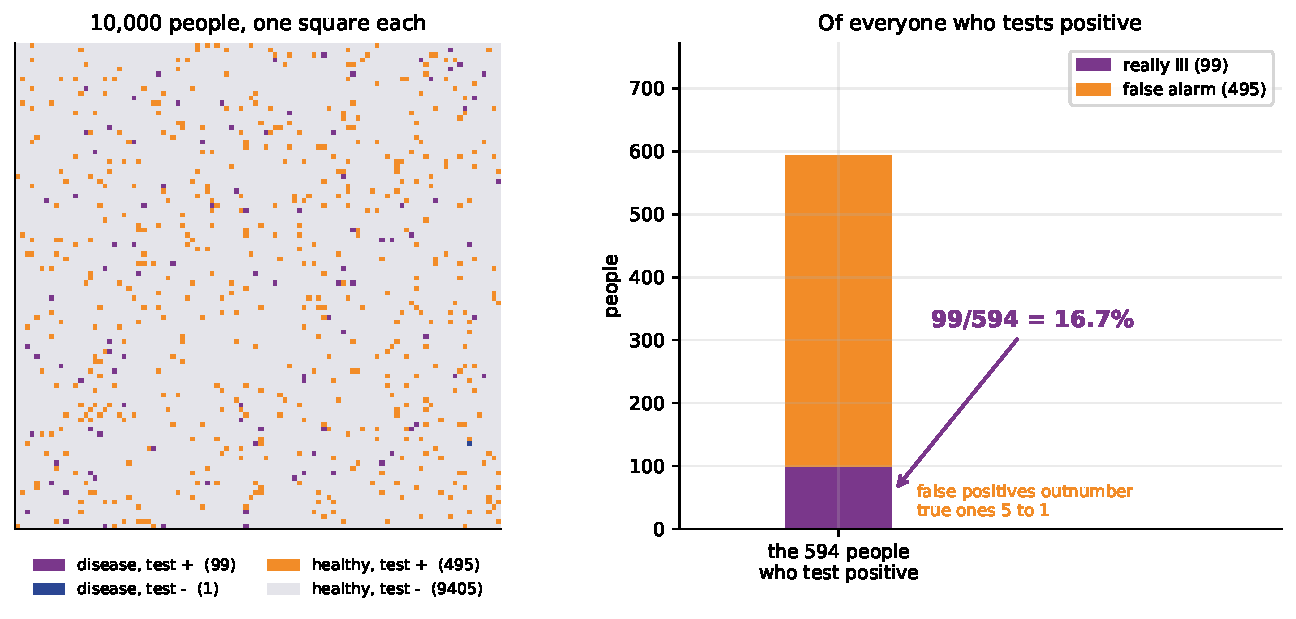
\includegraphics[width=0.82\textwidth]{basegrid.pdf}
  \end{center}
  \begin{center}\small
    Purple: ill and correctly flagged, $99$ of them. Orange: healthy and
    wrongly flagged, $495$. \textbf{The orange squares are what you cannot
    see when you only look at the test's accuracy figures} --- and they are
    five times as numerous as the purple ones.
  \end{center}
\end{frame}

\begin{frame}[fragile,shrink=6]{And confirmed in code, two ways}
\begin{lstlisting}
PREV, SENS, SPEC = 0.01, 0.99, 0.95
num = SENS * PREV                              # P(+, D)
den = SENS * PREV + (1 - SPEC) * (1 - PREV)    # P(+)
print(num / den)
\end{lstlisting}
\begin{outblk}
joint  P(+, D)    = P(+|D) P(D)       = 0.99 * 0.01 = 0.009900
joint  P(+, notD) = P(+|notD) P(notD) = 0.05 * 0.99 = 0.049500
evidence P(+)     = 0.009900 + 0.049500 = 0.059400
POSTERIOR P(D|+)  = 0.009900 / 0.059400 = 0.166667   = 16.6667%
exact fraction    = 99/594 = 1/6 ?  True
\end{outblk}
\onslide<2->
\begin{outblk}
confirmed by simulation, 2,000,000 people, seed 0
   simulated P(D|+) = 0.165611   analytic 0.166667   difference 0.001055
\end{outblk}
\onslide<3->
\begin{center}\small
  Two million simulated people agree with the algebra to $0.001$.
  \textbf{The result is not a trick of the formula; it is what actually
  happens to the population.}
\end{center}
\end{frame}

\begin{frame}[fragile,shrink=10]{What would make the test useful?}
\begin{columns}[T]
  \begin{column}{0.44\textwidth}
\begin{outblk}
prevalence  P(D|+)
    0.001  0.0194
    0.010  0.1667
    0.050  0.5103
    0.200  0.8319
    0.500  0.9519
specificity P(D|+)  (prev. 1%)
   0.9000  0.0909
   0.9500  0.1667
   0.9900  0.5000
   0.9990  0.9091
   0.9999  0.9901
\end{outblk}
  \end{column}
  \begin{column}{0.54\textwidth}
    \begin{block}{Raise the prior}
      \footnotesize Test people with symptoms rather than everybody. At
      $20\%$ prevalence the same test gives $0.8319$. \textbf{Screening a
      population is a different problem from testing a patient who walked in
      complaining.}
    \end{block}
    \begin{alertblock}{Or raise the \emph{specificity} --- not the
    sensitivity}
      \footnotesize $95\% \to 99.9\%$ specificity takes the posterior from
      $0.1667$ to $\mathbf{0.9091}$. \textbf{On a rare condition, false
      positives are the entire problem.}
    \end{alertblock}
  \end{column}
\end{columns}
\vspace{0.2em}
\begin{center}
  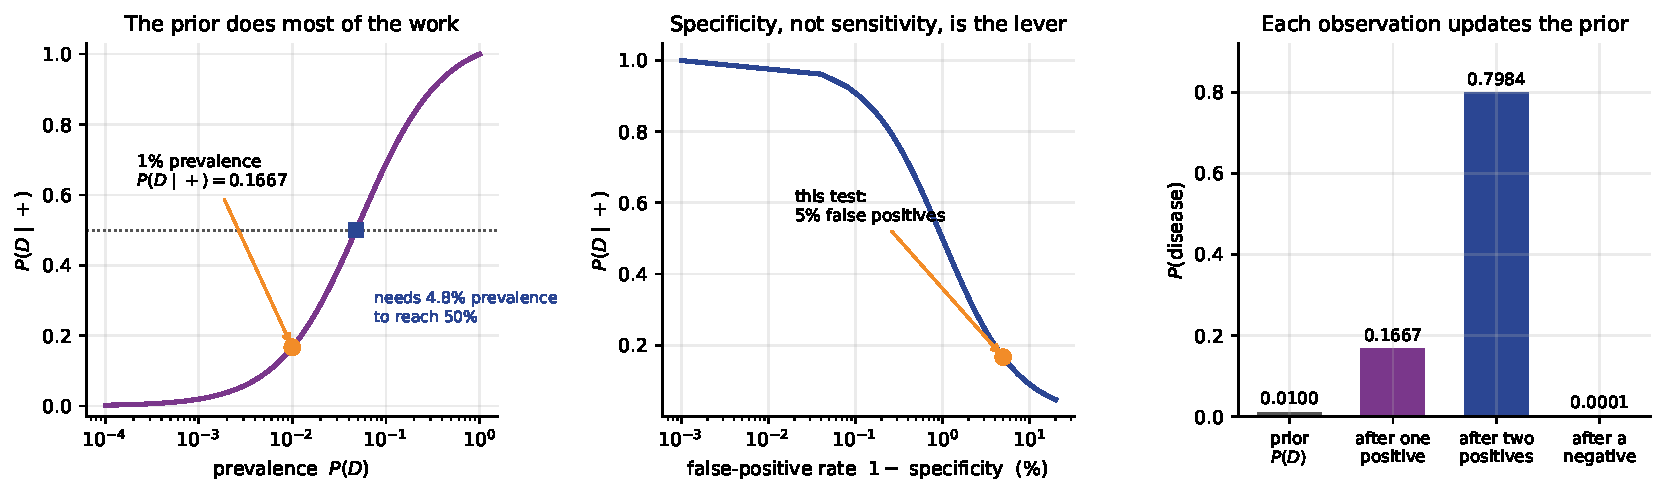
\includegraphics[width=0.80\textwidth]{prevalence.pdf}
\end{center}
\begin{center}\footnotesize
  You need $4.8\%$ prevalence before a positive result is an even-money bet.
  Right-hand panel: \textbf{yesterday's posterior is today's prior} --- test
  twice and $0.1667$ becomes $0.7984$; a negative takes it to $0.0001$.
\end{center}
\end{frame}

% =====================================================================
\section[MAP and ML]{Two decision rules: MAP and ML}
\label{sec:decide}

\begin{frame}[fragile,shrink=9]{Two rules, one piece of evidence, opposite
answers}
\begin{columns}[T]
  \begin{column}{0.48\textwidth}
    \begin{block}{Maximum likelihood (ML)}
      \small $\hat{c}_{\text{ML}} = \arg\max_{c} P(x \mid c)$ ---
      ``which class explains the evidence best?'' Ignores how common the
      classes are.
    \end{block}
  \end{column}
  \begin{column}{0.48\textwidth}
    \begin{block}{Maximum a posteriori (MAP)}
      \small $\hat{c}_{\text{MAP}} = \arg\max_{c} P(x \mid c)P(c)$ ---
      ``which class is most probable?'' This is what a classifier uses.
      ($P(x)$ is dropped: it cannot change the winner.)
    \end{block}
  \end{column}
\end{columns}
\vspace{0.2em}
\begin{outblk}
MAP against ML on the same evidence
   ML  rule: argmax P(+|c)      -> P(+|D)=0.9900 vs P(+|notD)=0.0500  -> says DISEASE
   MAP rule: argmax P(+|c)P(c)  -> 0.009900 vs 0.049500  -> says NO DISEASE
   the prior ratio is 99:1 against; the likelihood ratio is only 19.8:1 in favour
\end{outblk}
\onslide<2->
\begin{alertblock}{Read the last line slowly}
  \footnotesize The evidence is $19.8$ times more consistent with disease
  than with health. That is genuinely strong evidence. \textbf{It is not
  strong enough}, because it starts $99$ to $1$ behind.
  $19.8 < 99$, so the posterior odds are still against.
\end{alertblock}
\onslide<3->
\begin{center}\small
  Posterior odds $=$ likelihood ratio $\times$ prior odds:
  $\;\dfrac{1}{5} = 19.8 \times \dfrac{1}{99}$.
  \textbf{One multiplication, and it is the whole of Bayesian updating.}
\end{center}
\end{frame}

% =====================================================================
\section[Naive assumption]{From Bayes' theorem to a classifier}
\label{sec:naive}

\begin{frame}[fragile,shrink=9]{Predict first \#2}
An instance is a vector $x = (x_1, \ldots, x_d)$, so
$\hat{c} = \arg\max_{c} P(c)\,P(x_1, \ldots, x_d \mid c)$. But
$P(x_1,\ldots,x_d \mid c)$ is a probability for \emph{every combination} of
feature values: with $d$ binary features, a table of $2^d$ cells per class,
$C\,(2^{d}-1)$ free parameters, every one estimated from data.

\begin{center}
  \textbf{At $d = 30$ --- fewer features than \texttt{breast\_cancer} has ---
  how many is that? And how many rows do you have?}
\end{center}
\vspace{0.2em}
\onslide<2->
\begin{outblk}
d binary features, 2 classes
    d        joint  C(2^d - 1)     naive  C*d            ratio
    3                       14              6                2
    5                       62             10                6
   10                    2,046             20              102
   20                2,097,150             40           52,429
   30            2,147,483,646             60       35,791,394
   64 36,893,488,147,419,103,230            128 288,230,376,151,711,744
\end{outblk}
\onslide<3->
\begin{alertblock}{Two billion parameters, five hundred and sixty-nine rows}
  \footnotesize \texttt{breast\_cancer} has $569$ patients. The joint table at
  $d=30$ has $2{,}147{,}483{,}646$ free parameters. \textbf{You have about
  one row for every four million parameters.} At $d = 64$ ---
  \texttt{load\_digits}, one bit per pixel --- the joint table has more cells
  than there are grains of sand on Earth.
\end{alertblock}
\end{frame}

\begin{frame}[shrink=8]{Drawn: exponential against linear}
  \begin{center}
    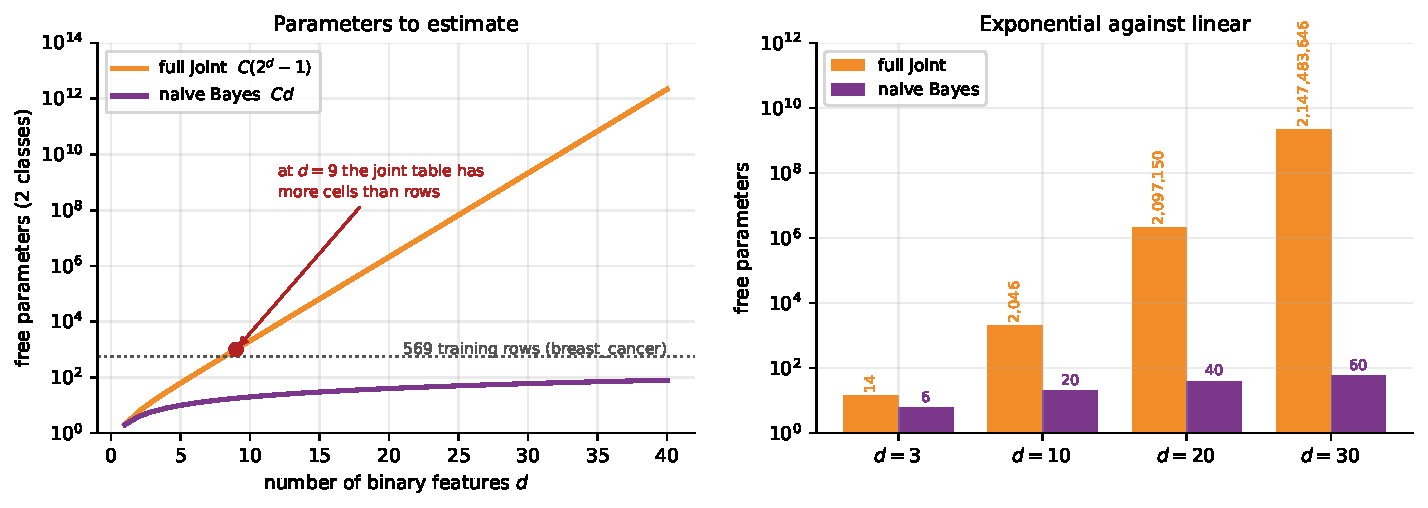
\includegraphics[width=0.88\textwidth]{params.pdf}
  \end{center}
  \begin{center}\small
    The joint table passes the $569$ available training rows at
    \textbf{$d = 9$}. Nine binary features. \textbf{Everything past that
    point is a table you cannot fill}, and the naive line --- the purple one
    --- is the only thing on the plot that stays inside your data budget.
  \end{center}
\end{frame}

\begin{frame}[shrink=4]{The naive assumption, stated precisely}
  \begin{exampleblock}{Conditional independence given the class}
    \centering
    \[
      P(x_1, x_2, \ldots, x_d \mid c)
        \;=\; \prod_{j=1}^{d} P(x_j \mid c)
    \]
    \small Equivalently: \emph{once you know the class}, knowing one feature
    tells you nothing about any other.
    $P(x_i \mid c, x_j) = P(x_i \mid c)$ for all $i \neq j$.
  \end{exampleblock}
  \begin{center}\small
  \begin{tabular}{@{}ll@{}}
    \toprule
    \textbf{What it does \emph{not} say} & \textbf{What it does say}\\
    \midrule
    the features are independent & they are independent \emph{within each
      class}\\
    \emph{outlook} and \emph{humidity} are unrelated & they are unrelated
      \emph{among the days you played}\\
    \bottomrule
  \end{tabular}
  \end{center}
  \begin{alertblock}{}
    \centering\footnotesize
    \textbf{It is almost always false.} It is made anyway, because it is the
    difference between $2^d$ parameters and $d$ of them --- and because, as we
    shall measure, the resulting classifier is often right even when its
    probabilities are not.
  \end{alertblock}
\end{frame}

\begin{frame}[fragile,shrink=7]{What the assumption buys, on one concrete table}
Fourteen weather records. \texttt{Outlook} has $3$ levels,
\texttt{Temperature} $3$, \texttt{Humidity} $2$, \texttt{Wind} $2$;
two classes.
\begin{outblk}
the tennis table: outlook(3) temperature(3) humidity(2) wind(2), 2 classes
   full joint        70 free parameters (a 36-cell table per class)
   naive Bayes       12 free parameters + 1 for the prior
   training rows available: 14
   rows per joint cell on average: 0.194
\end{outblk}
\onslide<2->
\begin{columns}[T]
  \begin{column}{0.48\textwidth}
    \begin{block}{The joint way}
      \footnotesize $3\times3\times2\times2 = 36$ cells per class, $70$ free
      parameters in all. With $14$ rows you get \textbf{$0.194$ rows per
      cell}: most cells are empty and most probabilities are $0$.
    \end{block}
  \end{column}
  \begin{column}{0.48\textwidth}
    \begin{alertblock}{The naive way}
      \footnotesize $(3-1)+(3-1)+(2-1)+(2-1) = 6$ per class, so
      $\mathbf{12}$ plus one prior. \textbf{Every one of them is estimated
      from at least five rows.} That is the trade: a wrong model you can fit
      against a right model you cannot.
    \end{alertblock}
  \end{column}
\end{columns}
\end{frame}

\begin{frame}[shrink=5]{The naive Bayes classifier, complete}
  \begin{exampleblock}{}
    \centering
    \[
      \hat{c} \;=\; \arg\max_{c \in \mathcal{C}} \;
        P(c) \prod_{j=1}^{d} P(x_j \mid c)
    \]
  \end{exampleblock}
  \begin{center}\small
  \begin{tabular}{@{}lll@{}}
    \toprule
    \textbf{Quantity} & \textbf{Estimated as} & \textbf{Called}\\
    \midrule
    $P(c)$ & $N_c / N$ & the class prior\\
    $P(x_j \mid c)$, categorical & $N_{jc}(x_j) / N_c$ &
      \texttt{CategoricalNB}\\
    $P(x_j \mid c)$, word counts & $(T_{cw}) / \sum_{w'} T_{cw'}$ &
      \texttt{MultinomialNB}\\
    $P(x_j \mid c)$, continuous & $\mathcal{N}(x_j; \mu_{jc},
      \sigma^2_{jc})$ & \texttt{GaussianNB}\\
    \bottomrule
  \end{tabular}
  \end{center}
  \begin{center}\small
    \textbf{Training is counting.} There is no iteration, no gradient, no
    hyperparameter to search except the smoothing constant. On
    \texttt{digits} it fits in $1.23$\,ms against logistic regression's
    $127.78$\,ms.
  \end{center}
\end{frame}

% =====================================================================
\section[By hand]{Naive Bayes worked entirely by hand}
\label{sec:hand}

\begin{frame}[shrink=9]{The fourteen rows}
\begin{center}\scriptsize
\begin{tabular}{@{}rllllc@{}}
  \toprule
  \# & Outlook & Temperature & Humidity & Wind & \textbf{Play}\\
  \midrule
  1 & Sunny & Hot & High & Weak & No\\
  2 & Sunny & Hot & High & Strong & No\\
  3 & Overcast & Hot & High & Weak & Yes\\
  4 & Rain & Mild & High & Weak & Yes\\
  5 & Rain & Cool & Normal & Weak & Yes\\
  6 & Rain & Cool & Normal & Strong & No\\
  7 & Overcast & Cool & Normal & Strong & Yes\\
  8 & Sunny & Mild & High & Weak & No\\
  9 & Sunny & Cool & Normal & Weak & Yes\\
  10 & Rain & Mild & Normal & Weak & Yes\\
  11 & Sunny & Mild & Normal & Strong & Yes\\
  12 & Overcast & Mild & High & Strong & Yes\\
  13 & Overcast & Hot & Normal & Weak & Yes\\
  14 & Rain & Mild & High & Strong & No\\
  \bottomrule
\end{tabular}
\end{center}
\begin{center}\small
  Nine \emph{Yes}, five \emph{No}. Priors
  $P(\text{Yes}) = 9/14 = 0.642857$ and
  $P(\text{No}) = 5/14 = 0.357143$.
  \textbf{This is the table every Indian syllabus uses; learn it once.}
\end{center}
\end{frame}

\begin{frame}[shrink=9]{Step 1: the tables --- which is just counting}
\begin{center}\scriptsize
\begin{tabular}{@{}llrlrl@{}}
  \toprule
  \textbf{Feature} & \textbf{Level} & \multicolumn{2}{c}{\textbf{given Yes}
    ($N=9$)} & \multicolumn{2}{c}{\textbf{given No} ($N=5$)}\\
  \midrule
  Outlook & Overcast & 4/9 & $=0.4444$ & \textbf{0/5} & $=\mathbf{0.0000}$\\
          & Rain     & 3/9 & $=0.3333$ & 2/5 & $=0.4000$\\
          & Sunny    & 2/9 & $=0.2222$ & 3/5 & $=0.6000$\\
  \midrule
  Temperature & Cool & 3/9 & $=0.3333$ & 1/5 & $=0.2000$\\
              & Hot  & 2/9 & $=0.2222$ & 2/5 & $=0.4000$\\
              & Mild & 4/9 & $=0.4444$ & 2/5 & $=0.4000$\\
  \midrule
  Humidity & High   & 3/9 & $=0.3333$ & 4/5 & $=0.8000$\\
           & Normal & 6/9 & $=0.6667$ & 1/5 & $=0.2000$\\
  \midrule
  Wind & Strong & 3/9 & $=0.3333$ & 3/5 & $=0.6000$\\
       & Weak   & 6/9 & $=0.6667$ & 2/5 & $=0.4000$\\
  \bottomrule
\end{tabular}
\end{center}
\begin{center}\small
  Each block sums to $1$ down its column. \textbf{That is the entire
  training procedure.} Note the bold zero --- we come back to it in ten
  minutes.
\end{center}
\end{frame}

\begin{frame}[shrink=6]{Step 2: classify a new day, by hand}
  New instance: $x = (\text{Sunny}, \text{Cool}, \text{High},
  \text{Strong})$.
  \begin{columns}[T]
    \begin{column}{0.49\textwidth}
      \begin{block}{Score for \emph{No}}
        \small
        \begin{align*}
          &\tfrac{5}{14} \times \tfrac{3}{5} \times \tfrac{1}{5}
            \times \tfrac{4}{5} \times \tfrac{3}{5}\\
          &= 0.357143 \times 0.6 \times 0.2 \times 0.8 \times 0.6\\
          &= \mathbf{0.02057143}
        \end{align*}
      \end{block}
    \end{column}
    \begin{column}{0.49\textwidth}
      \begin{block}{Score for \emph{Yes}}
        \small
        \begin{align*}
          &\tfrac{9}{14} \times \tfrac{2}{9} \times \tfrac{3}{9}
            \times \tfrac{3}{9} \times \tfrac{3}{9}\\
          &= 0.642857 \times 0.2222 \times 0.3333^{3}\\
          &= \mathbf{0.00529101}
        \end{align*}
      \end{block}
    \end{column}
  \end{columns}
  \vspace{0.2em}
  \begin{center}\small
    Evidence $P(x) = 0.02057143 + 0.00529101 = 0.02586243$, so
    \[
      P(\text{No} \mid x) = \frac{0.02057143}{0.02586243} = \mathbf{0.795417},
      \qquad
      P(\text{Yes} \mid x) = \mathbf{0.204583}.
    \]
  \end{center}
  \begin{alertblock}{}
    \centering\small
    \textbf{Prediction: \emph{No}}, at posterior odds $3.8880 : 1$. Five
    multiplications and one division.
  \end{alertblock}
\end{frame}

\begin{frame}[shrink=8]{Drawn: the five factors and their product}
  \begin{center}
    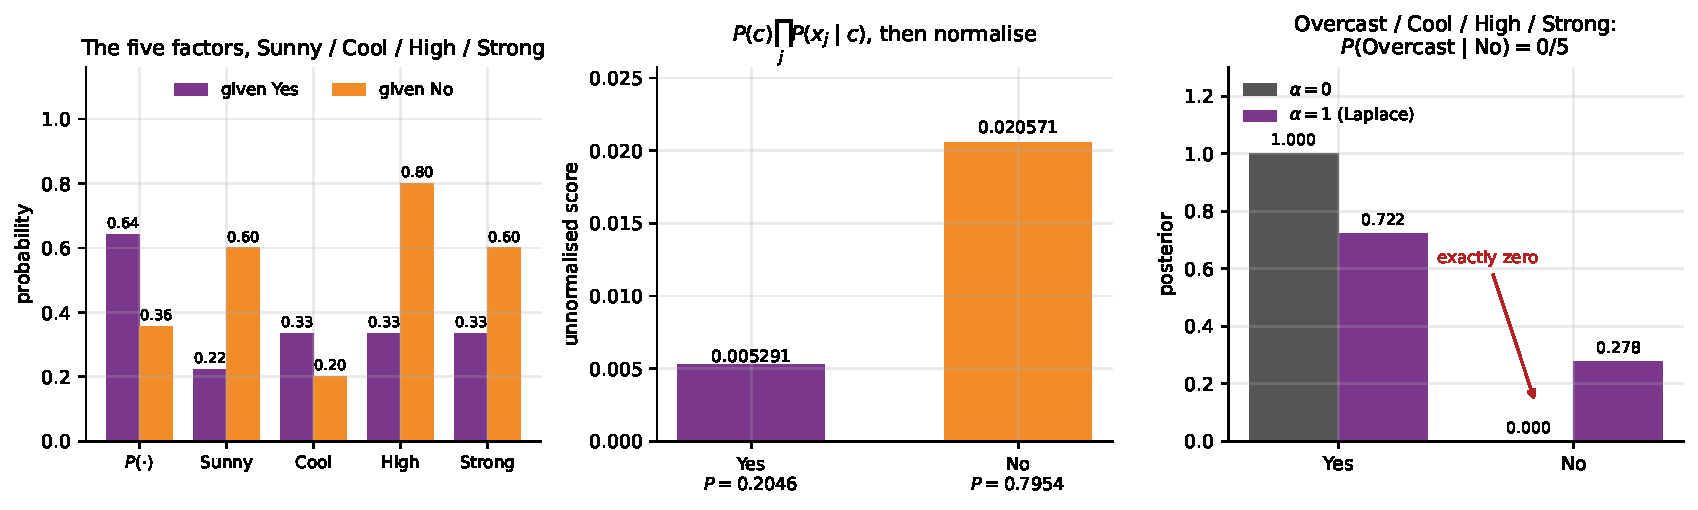
\includegraphics[width=0.94\textwidth]{tennis.pdf}
  \end{center}
  \begin{center}\small
    Left: the five numbers that get multiplied. \emph{High} humidity is the
    strongest single piece of evidence against playing ($0.80$ against
    $0.33$). Centre: their products, before normalising. Right: what happens
    when one factor is $0/5$ --- the next section.
  \end{center}
\end{frame}

\begin{frame}[fragile,shrink=6]{The identical result from scikit-learn}
\begin{lstlisting}
enc  = OrdinalEncoder(categories=LEVELS)
Xe   = enc.fit_transform(np.array(X_t, dtype=object))
cnb0 = CategoricalNB(alpha=1e-10, force_alpha=True).fit(Xe, ye)
cnb0.predict_proba(enc.transform([["Sunny","Cool","High","Strong"]]))
\end{lstlisting}
\begin{outblk}
the same instance through sklearn CategoricalNB(alpha=1e-10)
      predict_proba  No 0.795417   Yes 0.204583
      predict        No
      agrees with the hand calculation to 7.68e-12
\end{outblk}
\onslide<2->
\begin{outblk}
resubstitution accuracy of the hand model on all 14 rows
      13/14 = 0.9286
\end{outblk}
\onslide<3->
\begin{alertblock}{}
  \centering\footnotesize
  \textbf{There is nothing inside \texttt{CategoricalNB} that you did not
  just do with a pen.} Note $\alpha = 10^{-10}$: the library smooths by
  default, and to reproduce the textbook arithmetic you must turn it off. In
  a moment you will see why the default exists.
\end{alertblock}
\end{frame}

% =====================================================================
\section[Zero frequency]{The zero-frequency problem}
\label{sec:zero}

\begin{frame}[shrink=6]{One empty cell kills the whole product}
  Look again at the table: \textbf{\emph{Overcast} never appears with
  \emph{No}}. Four overcast days, all of them played.
  \[
    P(\text{Overcast} \mid \text{No}) = \frac{0}{5} = 0.
  \]
  \begin{center}\small
    Now classify $x = (\text{Overcast}, \text{Cool}, \text{High},
    \text{Strong})$. Three of the four features favour \emph{No}:
    \emph{High} humidity ($0.80$ against $0.33$), \emph{Strong} wind
    ($0.60$ against $0.33$), \emph{Cool} is near-neutral.
  \end{center}
  \begin{center}
    \small Score for \emph{No}:
    $\;\dfrac{5}{14} \times \mathbf{\dfrac{0}{5}} \times \dfrac{1}{5}
    \times \dfrac{4}{5} \times \dfrac{3}{5}$
  \end{center}
  \onslide<2->
  \begin{alertblock}{Predict first \#3: what is that product?}
    \centering
    \Large $\mathbf{0.00000000}$, so $P(\text{No} \mid x)$ is
    \textbf{exactly zero}.
  \end{alertblock}
\end{frame}

\begin{frame}[fragile,shrink=6]{``Impossible'', on the evidence of four
missing rows}
\begin{outblk}
classify ('Overcast', 'Cool', 'High', 'Strong') with alpha = 0
      P(No) * prod = 5/14 * 0/5 * 1/5 * 4/5 * 3/5 = 0.00000000
      P(Yes) * prod = 9/14 * 4/9 * 3/9 * 3/9 * 3/9 = 0.01058201
      P(Yes|x) = 1.000000   P(No|x) = 0.000000
      the other three factors for No were 1/5, 4/5, 3/5 -- none of them small.
\end{outblk}
\onslide<2->
\begin{alertblock}{A probability of exactly zero is a claim you cannot
defend}
  \footnotesize The model is not saying ``unlikely''. It is saying
  \textbf{impossible}: no amount of evidence from the other three features
  can ever recover it, because they are all multiplied by $0$. \textbf{One
  unobserved combination has vetoed the entire class.} And the sample size
  behind that veto is \emph{five rows}.
\end{alertblock}
\onslide<3->
\begin{center}\small
  Multiplication is unforgiving in a way that addition is not. This is the
  \textbf{zero-frequency problem}, and every naive Bayes implementation on
  earth ships with a fix turned on by default.
\end{center}
\end{frame}

\begin{frame}[shrink=6]{Laplace smoothing: pretend you saw one of everything}
  \begin{exampleblock}{}
    \centering
    \[
      \hat{P}(x_j = t \mid c) \;=\; \frac{N_{tjc} + \alpha}
        {N_c + \alpha\,n_j}
    \]
    \small where $n_j$ is the number of levels feature $j$ has, and
    $\alpha = 1$ is \emph{Laplace} (add-one) smoothing. $\alpha < 1$ is called
    \emph{Lidstone}.
  \end{exampleblock}
  \begin{center}\small
    \texttt{Outlook} has three levels, so for the \emph{No} class the
    denominator becomes $5 + 3 = 8$:
    \[
      P(\text{Overcast} \mid \text{No}) = \frac{0+1}{5+3}
        = \frac{1}{8} = 0.1250 .
    \]
  \end{center}
  \begin{center}\small
    \textbf{Add $\alpha$ to the top and $\alpha n_j$ to the bottom} --- so
    the column still sums to one. Getting the denominator wrong is the
    single commonest examination error on this topic.
  \end{center}
\end{frame}

\begin{frame}[fragile,shrink=7]{The same instance, smoothed: before and after}
\begin{outblk}
the same instance with Laplace alpha = 1
      P(No) * prod = 5/14 * 1/8 * 2/8 * 5/7 * 4/7 = 0.00455539
      P(Yes) * prod = 9/14 * 5/12 * 4/12 * 4/11 * 4/11 = 0.01180638
      P(Overcast|No) = (0+1)/(5+3) = 0.1250
      P(Yes|x) = 0.721583   P(No|x) = 0.278417
      'impossible' has become 27.84%
\end{outblk}
\onslide<2->
\begin{center}\small
\begin{tabular}{@{}lcc@{}}
  \toprule
   & $P(\text{No} \mid x)$ & $P(\text{Yes} \mid x)$\\
  \midrule
  $\alpha = 0$ & $\mathbf{0.000000}$ & $1.000000$\\
  $\alpha = 1$ & $\mathbf{0.278417}$ & $0.721583$\\
  \bottomrule
\end{tabular}
\end{center}
\onslide<3->
\begin{alertblock}{Check the denominators against the level counts}
  \footnotesize \texttt{Outlook} and \texttt{Temperature} have three levels,
  so $5+3 = 8$. \texttt{Humidity} and \texttt{Wind} have two, so $5+2 = 7$.
  For \emph{Yes}: $9+3 = 12$ and $9+2 = 11$. \textbf{Every fraction on that
  first line can be read straight off the level counts.}
\end{alertblock}
\end{frame}

\begin{frame}[fragile,shrink=8]{How much smoothing? Sweep $\alpha$ and watch}
\begin{outblk}
alpha sweep on the same instance
      alpha    P(No|x)   P(Yes|x)  prediction
       0.00   0.000000   1.000000  Yes
       0.01   0.006403   0.993597  Yes
       0.10   0.057749   0.942251  Yes
       1.00   0.278417   0.721583  Yes
       5.00   0.375650   0.624350  Yes
     100.00   0.360719   0.639281  Yes
   as alpha grows the conditionals wash out and the PRIOR takes over:
   P(Yes) = 9/14 = 0.6429, which is the limit above
\end{outblk}
\onslide<2->
\begin{center}\small
  $\alpha$ interpolates between \textbf{trust the counts completely}
  ($\alpha \to 0$) and \textbf{ignore the features entirely}
  ($\alpha \to \infty$, where the posterior is the prior $9/14 = 0.6429$).
  It is a regularisation parameter, and like every regularisation parameter
  it is chosen by cross-validation.
\end{center}
\end{frame}

\begin{frame}[shrink=8]{Drawn: what $\alpha$ does, on a table and on text}
  \begin{center}
    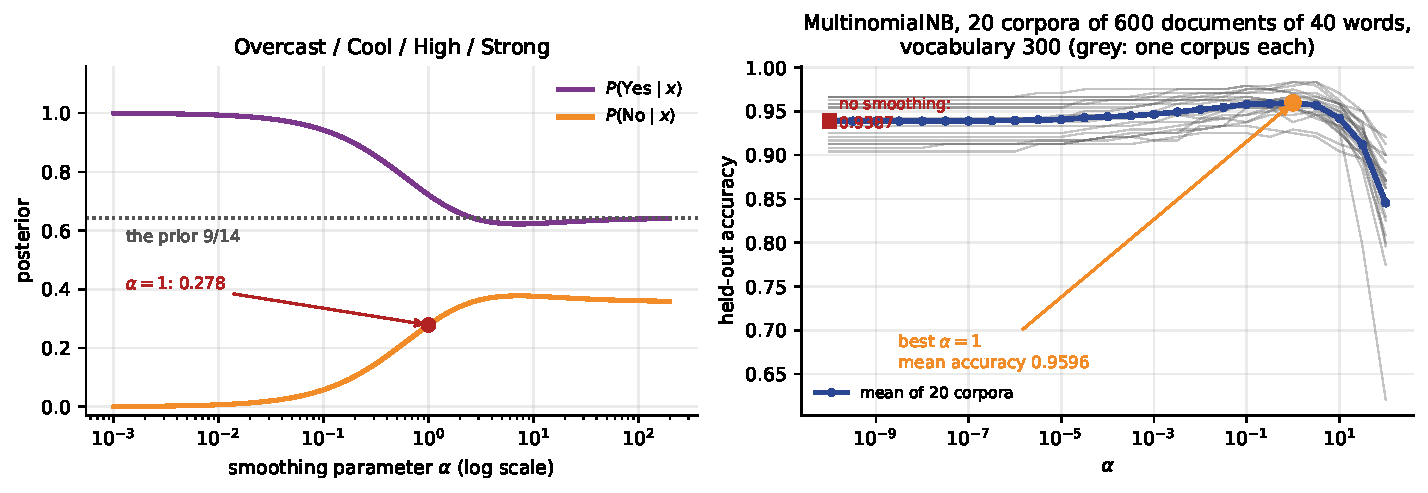
\includegraphics[width=0.90\textwidth]{smoothing.pdf}
  \end{center}
  \begin{center}\small
    Left: the tennis posterior as $\alpha$ sweeps from $0$ to $200$ ---
    starting at the indefensible $0$ and flattening onto the prior $9/14$.
    Right: held-out accuracy of \texttt{MultinomialNB}, averaged over
    \textbf{twenty} corpora of $600$ synthetic documents (grey: one corpus
    each --- look how far one draw can wander). \textbf{No smoothing gives
    $0.9387$; the best $\alpha$, which is $1$, gives $0.9596$}, and too much
    costs more than too little: $\alpha = 100$ falls to $0.8454$.
    \textbf{$\alpha$ is a hyperparameter, so cross-validate it --- and not
    on one split.}
  \end{center}
\end{frame}

\begin{frame}[fragile,shrink=7]{Reported honestly: on \emph{this} table the
label never flips}
\begin{outblk}
how many of the 36 possible days contain a zero, and how many flip?
   36 possible days; 12 of them make one class exactly impossible (33.3%)
   smoothing changes the prediction on 0 of the 36
mean |change| in P(Yes|x) across all 36 days when alpha goes 0 -> 1
   mean 0.0942   max 0.4356
\end{outblk}
\onslide<2->
\begin{alertblock}{Say the honest thing, not the convenient thing}
  \footnotesize A third of all possible days drive one class to exactly zero.
  But the \emph{argmax} never changes here, because every zero falls on
  \emph{No} --- the minority class, which was losing anyway. \textbf{What
  smoothing fixes on this table is the posterior, not the label}: on average
  it moves $P(\text{Yes} \mid x)$ by $0.0942$ and at worst by $0.4356$.
\end{alertblock}
\onslide<3->
\begin{center}\small
  \textbf{On text the label does flip}, because there the zeros land on both
  classes at once --- which is the next slide.
\end{center}
\end{frame}

% =====================================================================
\section[Logs]{Text, log-probabilities and underflow}
\label{sec:logs}

\begin{frame}[fragile,shrink=8]{A twelve-message spam corpus, built inline}
\begin{lstlisting}
SPAM = ["win a free laptop click this link now",
        "congratulations you win a free prize click now", ...]
HAM  = ["the lecture notes for the machine learning class are on the portal",
        "please submit your assignment before the deadline on friday", ...]
\end{lstlisting}
\begin{outblk}
12 messages (6 spam, 6 ham), vocabulary of 51 words
total word tokens: spam 46, ham 58
   word             n(spam)  n(ham)    P(w|S)    P(w|H)  log ratio
   free                   7       0   0.08247   0.00917     2.1961
   click                  6       0   0.07216   0.00917     2.0625
   win                    4       0   0.05155   0.00917     1.7261
   the                    1      11   0.02062   0.11009    -1.6751
   on                     0       3   0.01031   0.03670    -1.2697
   notes                  0       2   0.01031   0.02752    -0.9820
\end{outblk}
\onslide<2->
\begin{center}\small
  With $\alpha = 1$ and $V = 51$:
  $P(\text{free} \mid S) = (7+1)/(46+51) = 8/97 = 0.08247$ and
  $P(\text{free} \mid H) = (0+1)/(58+51) = 1/109 = 0.00917$.
  \textbf{Every word becomes a weight, and classifying is adding them up.}
\end{center}
\end{frame}

\begin{frame}[fragile,shrink=6]{By hand: score ``click the free link''}
\begin{outblk}
      log P(S)  = log 0.5000 = -0.693147
      log P(H)  = log 0.5000 = -0.693147
      click    P(w|S)=0.07216 log=-2.6288   P(w|H)=0.00917 log=-4.6913
      free     P(w|S)=0.08247 log=-2.4953   P(w|H)=0.00917 log=-4.6913
      link     P(w|S)=0.04124 log=-3.1884   P(w|H)=0.00917 log=-4.6913
      the      P(w|S)=0.02062 log=-3.8816   P(w|H)=0.11009 log=-2.2064
      total log score  spam -12.887198   ham -16.973632
      P(spam|msg) = 0.983479   P(ham|msg) = 0.016521
\end{outblk}
\onslide<2->
\begin{outblk}
   sklearn MultinomialNB(alpha=1)  ham 0.016521  spam 0.983479
   agreement to 8.88e-16
\end{outblk}
\onslide<3->
\begin{center}\small
  Add five numbers, compare two totals. The margin is
  $-12.887198 - (-16.973632) = 4.086434$, and
  $1/(1 + e^{-4.086434}) = 0.983479$. \textbf{``The'' argues for ham and
  loses, three to one.}
\end{center}
\end{frame}

\begin{frame}[shrink=8]{Drawn: every word is a weight}
  \begin{center}
    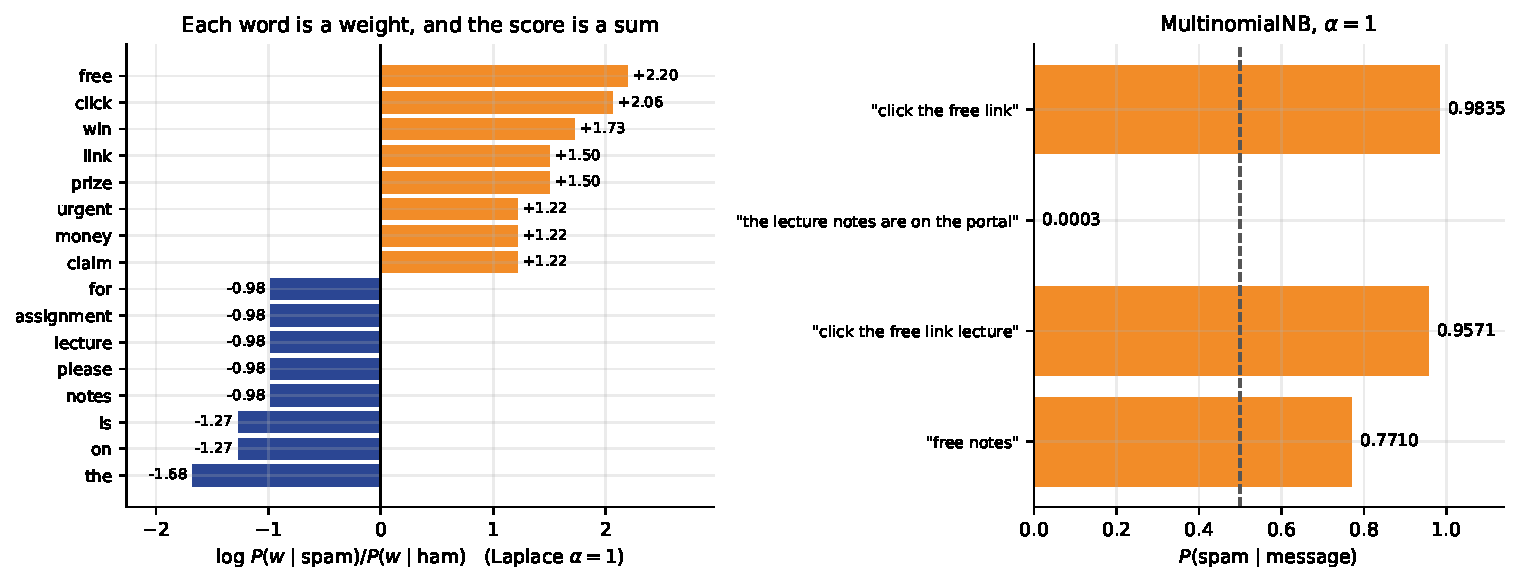
\includegraphics[width=0.88\textwidth]{spam.pdf}
  \end{center}
  \begin{center}\small
    Left: $\log P(w \mid S)/P(w \mid H)$ for the sixteen most opinionated
    words. Right: four messages scored. \textbf{``Click the free link
    lecture'' still scores $0.9571$} --- one ham word cannot overturn three
    spam words, which is exactly what \emph{summing} evidence should do, and
    exactly what a raw product cannot do.
  \end{center}
\end{frame}

\begin{frame}[fragile,shrink=7]{Why we took logs at all: watch it underflow}
Synthetic text: $600$ documents, vocabulary $400$, two classes sharing
$88\%$ of their vocabulary. Per-word probabilities run from
$3.6\times10^{-5}$ to $2.4\times10^{-2}$.

\begin{center}
  \textbf{Predict first \#4: multiply them one token at a time. At how many
  tokens does the running product become \emph{exactly} $0.0$?}
\end{center}
\onslide<2->
\begin{outblk}
     tokens      raw product      sum of logs       exp(sum)
          1     6.868132e-03          -4.9809   6.868132e-03
         20     2.625046e-41         -93.4409   2.625046e-41
        100    7.423356e-226        -518.3796  7.423356e-226
        120    2.511950e-270        -620.7769  2.511950e-270
        200     0.000000e+00       -1023.0046   0.000000e+00
        400     0.000000e+00       -2050.9589   0.000000e+00
   the raw product first becomes EXACTLY 0.0 at 148 tokens
\end{outblk}
\onslide<3->
\begin{alertblock}{$\mathbf{148}$ tokens}
  \footnotesize About one short paragraph. A real e-mail, a review, a support
  ticket --- \textbf{all longer than that}. The smallest positive
  \texttt{float64} is $4.9\times10^{-324}$, and a product of $148$ numbers
  averaging $10^{-3}$ walks straight past it.
\end{alertblock}
\end{frame}

\begin{frame}[shrink=8]{Drawn: the product dies, the sum does not}
  \begin{center}
    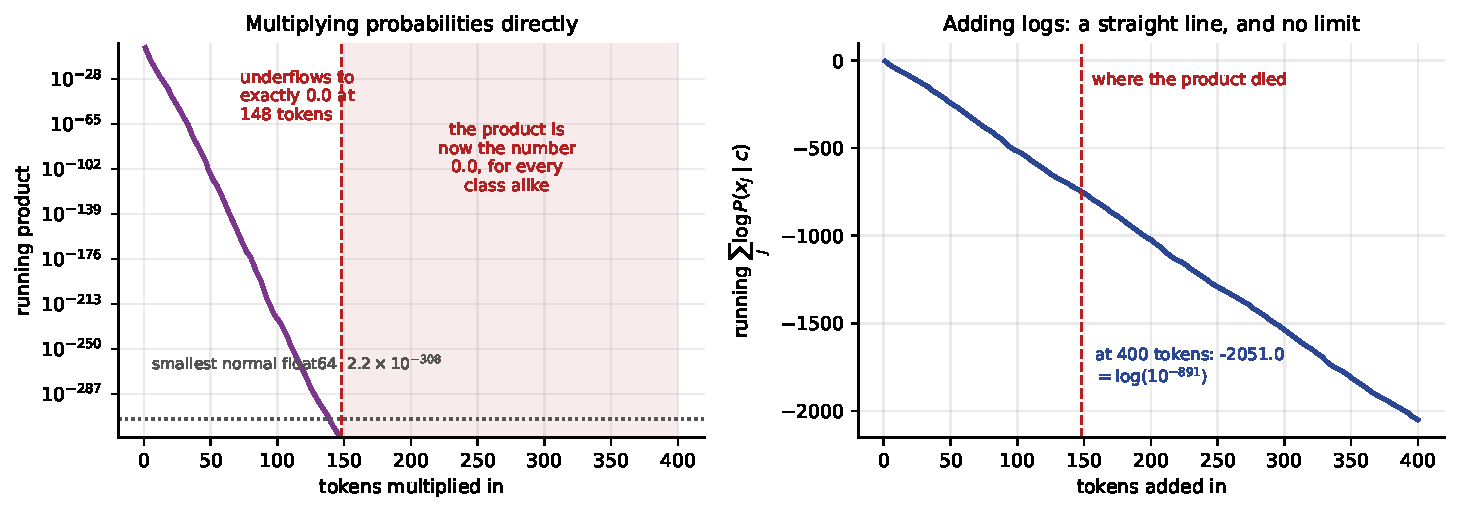
\includegraphics[width=0.88\textwidth]{underflow.pdf}
  \end{center}
  \begin{center}\small
    Left: the running product on a log axis, falling off the bottom of
    \texttt{float64} at token $148$. Right: the same computation as a sum of
    logs --- \textbf{a straight line with no floor at all}. At $400$ tokens
    it reads $-2051.0$, which is $\log(10^{-891})$: a number no
    floating-point format can hold, computed without difficulty.
  \end{center}
\end{frame}

\begin{frame}[fragile,shrink=7]{And it is not a cosmetic problem}
Score the whole test set twice --- once by multiplying, once by adding logs.
Documents are lengthened by tiling, the way an e-mail thread grows.
\begin{outblk}
    tokens  both scores 0.0  one score 0.0  raw-product acc  log acc
       120                0              0           0.9722   0.9722
       240              180              0           0.5056   0.9722
       360              180              0           0.5056   0.9722
       480              180              0           0.5056   0.9722
\end{outblk}
\onslide<2->
\begin{alertblock}{$0.9722 \rightarrow 0.5056$, and not one error message}
  \footnotesize At $240$ tokens, \textbf{all $180$ test documents} have both
  class scores equal to $0.0$. The comparison \texttt{0.0 > 0.0} is
  \texttt{False}, so every one of them is silently assigned to class $0$.
  \textbf{The accuracy halves and the program does not complain.}
\end{alertblock}
\onslide<3->
\begin{center}\small
  This is why \texttt{predict\_log\_proba} exists, why sklearn's naive Bayes
  classes store \texttt{feature\_log\_prob\_} rather than probabilities, and
  why you should be suspicious of any product of more than about a hundred
  probabilities.
\end{center}
\end{frame}

\begin{frame}[fragile,shrink=6]{Getting back to a probability: log-sum-exp}
The argmax needs only the log scores. If you want a posterior that sums to
one, you must exponentiate --- carefully.
\begin{outblk}
   logs [-800. -802.]
   naive  exp(a).sum() = 0.0000e+00  -> log = -inf
   stable mx + log(sum(exp(a-mx))) = -799.873072
\end{outblk}
\onslide<2->
\[
  \log \sum_k e^{a_k}
    \;=\; a_{\max} + \log \sum_k e^{\,a_k - a_{\max}}
\]
\begin{center}\small
  Subtracting the maximum makes the largest exponent exactly $e^0 = 1$, so
  nothing overflows and the biggest term never underflows. \textbf{The
  identity is exact --- it is just $\log(e^{a_{\max}} \sum e^{a-a_{\max}})$.}
\end{center}
\begin{alertblock}{}
  \centering\footnotesize
  \texttt{scipy.special.logsumexp} does this for you, and it is the same
  trick that makes \texttt{softmax} numerically safe in every neural-network
  library. You will meet it again in Lecture 17.
\end{alertblock}
\end{frame}

% =====================================================================
\section[Gaussian NB]{Gaussian naive Bayes: continuous features}
\label{sec:gauss}

\begin{frame}[shrink=6]{What do you count when the feature is a real number?}
  \begin{alertblock}{You cannot}
    \small \emph{Petal width} $=1.7$\,cm appears in the training set exactly
    zero times, or once. Counting gives you $0$ or $1/50$, and neither is
    useful.
  \end{alertblock}
  \begin{exampleblock}{So model the density instead}
    \[
      P(x_j \mid c) \;=\; \frac{1}{\sqrt{2\pi\sigma_{jc}^{2}}}
        \exp\!\left(-\frac{(x_j - \mu_{jc})^{2}}{2\sigma_{jc}^{2}}\right)
    \]
    \small One mean and one variance per feature per class, both estimated by
    maximum likelihood --- that is, the ordinary sample mean and the
    ordinary (biased, $\div N$) sample variance.
  \end{exampleblock}
  \begin{center}\small
    \textbf{Two parameters replace a whole histogram.} And note $P(x_j \mid
    c)$ is now a \emph{density}, which can exceed $1$; that is legal, and it
    normalises away when you divide by the evidence.
  \end{center}
\end{frame}

\begin{frame}[fragile,shrink=7]{By hand: one iris flower, one measurement}
\begin{outblk}
load_iris, petal width (cm), by class
   class          n      mean   sd (ML)
   setosa        50    0.2460    0.1043
   versicolor    50    1.3260    0.1958
   virginica     50    2.0260    0.2719
\end{outblk}
A flower with petal width $1.7$\,cm. Substitute into the density:
\begin{outblk}
      p(x|setosa     ) = 2.533257e-42   P(setosa|x) = 0.000000
      p(x|versicolor ) = 3.285675e-01   P(versicolor|x) = 0.314834
      p(x|virginica  ) = 7.150527e-01   P(virginica|x) = 0.685166
      PREDICTION: virginica
\end{outblk}
\onslide<2->
\begin{center}\small
  Priors are equal ($50$ of each), so the posterior is just the densities
  normalised: $0.7150527 / (0.3285675 + 0.7150527 + \text{tiny})
  = 0.685166$. \textbf{And \texttt{GaussianNB().predict\_proba([[1.7]])}
  returns \texttt{[0.\ \ 0.3148\ 0.6852]}.}
\end{center}
\end{frame}

\begin{frame}[shrink=8]{Drawn: three Gaussians and the boundaries they imply}
  \begin{center}
    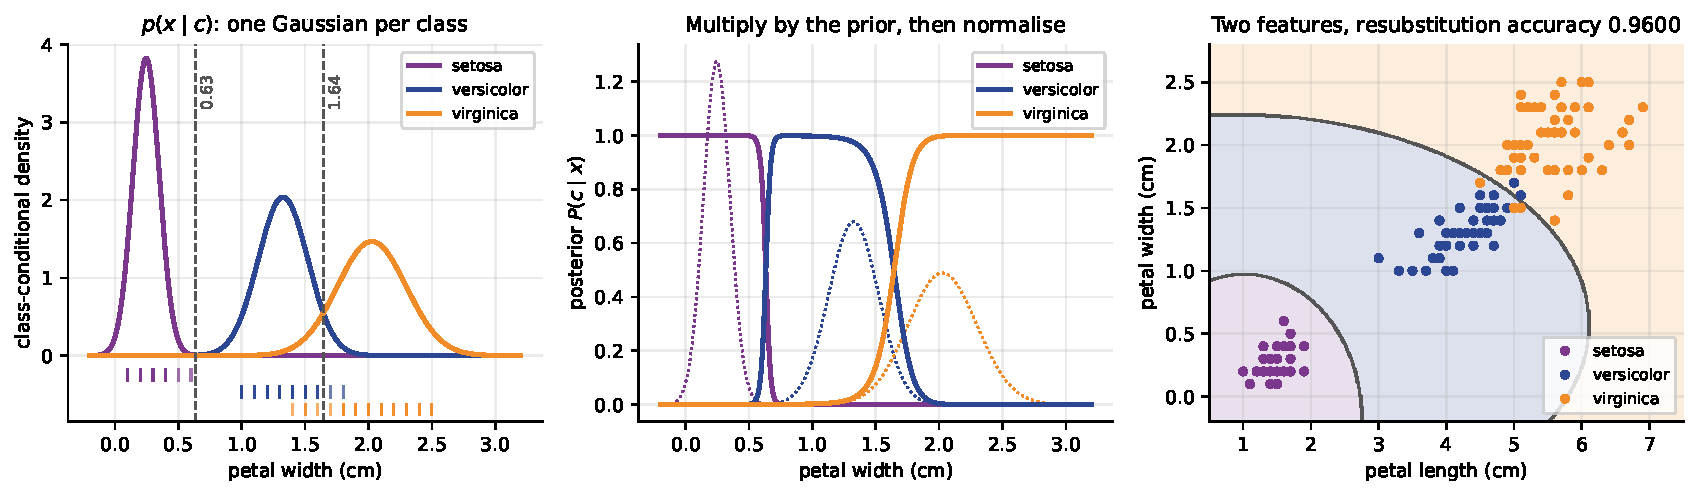
\includegraphics[width=0.92\textwidth]{gaussnb.pdf}
  \end{center}
  \begin{center}\small
    Left: one fitted Gaussian per class over petal width, with the raw
    measurements as ticks below. The two decision boundaries sit at
    \textbf{$0.6333$ and $1.6437$\,cm} --- solved numerically, exactly where
    the curves cross once the priors are applied. Centre: the posteriors.
    Right: two features, resubstitution accuracy $0.9600$.
  \end{center}
\end{frame}

\begin{frame}[fragile,shrink=7]{How good is it? Measured against two harder
models}
\begin{outblk}
GaussianNB against two others, 5-fold, on four bundled datasets
   dataset           GaussianNB    LogReg  RandForest  fit ms NB  fit ms LR
   iris                  0.9600    0.9600      0.9400       0.45       1.69
   wine                  0.9719    0.9832      0.9719       0.41       1.82
   breast_cancer         0.9385    0.9789      0.9649       0.53       2.40
   digits                0.8508    0.9694      0.9733       1.29     128.02

   dataset            rows x cols  NB passes  LR L-BFGS iterations
   iris                   150 x 4          1                    17
   wine                  178 x 13          1                    15
   breast_cancer         569 x 30          1                    19
   digits               1797 x 64          1                    32
\end{outblk}
\onslide<2->
\begin{columns}[T]
  \begin{column}{0.48\textwidth}
    \begin{block}{Competitive, not best}
      \footnotesize It ties logistic regression on \texttt{iris}, matches the
      random forest on \texttt{wine}, and gives away four points on
      \texttt{breast\_cancer} and twelve on \texttt{digits} --- where
      neighbouring pixels are heavily dependent.
    \end{block}
  \end{column}
  \begin{column}{0.48\textwidth}
    \begin{alertblock}{Quote the passes, not the milliseconds}
      \footnotesize \textbf{One pass against $32$ L-BFGS iterations} on
      \texttt{digits}. Naive Bayes has \emph{no} iterative solver: it reads
      the data once, accumulates sums and sums of squares, and stops. The
      \texttt{fit ms} columns measure this laptop on this afternoon and
      reproduce nowhere; the pass counts are the same everywhere.
    \end{alertblock}
  \end{column}
\end{columns}
\end{frame}

% =====================================================================
\section[Bad probabilities]{A good classifier and a bad probability
estimator}
\label{sec:calib}

\begin{frame}[fragile,shrink=7]{Predict first \#5}
\texttt{breast\_cancer}, $60/40$ split. \texttt{GaussianNB} scores $0.9342$
on the held-out patients; logistic regression scores $0.9649$.

\begin{center}
  \textbf{Take every prediction naive Bayes makes and read off how confident
  it says it is. What is the \emph{average} of those confidences?}
\end{center}
\vspace{0.2em}
\onslide<2->
\begin{outblk}
   GaussianNB           fraction with max-probability > 0.99 : 0.9649
                        fraction with max-probability > 0.999: 0.9298
                        fraction in [0.1, 0.9]              : 0.0219
                        mean confidence 0.9936 against accuracy 0.9342
   LogisticRegression   fraction with max-probability > 0.99 : 0.7105
                        fraction with max-probability > 0.999: 0.4956
                        fraction in [0.1, 0.9]              : 0.1360
                        mean confidence 0.9626 against accuracy 0.9649
\end{outblk}
\onslide<3->
\begin{alertblock}{$\mathbf{0.9936}$ confident, $\mathbf{0.9342}$ right}
  \footnotesize $93\%$ of its answers claim a probability above
  \textbf{$0.999$}, and only $2\%$ of them land anywhere between $0.1$ and
  $0.9$. Logistic regression's mean confidence, $0.9626$, sits essentially on
  top of its accuracy, $0.9649$. \textbf{One of these models knows what it
  does not know.}
\end{alertblock}
\end{frame}

\begin{frame}[fragile,shrink=8]{Where the claims and the reality part company}
\begin{outblk}
reliability: bin the predictions and compare claim with reality
   GaussianNB
      bin               n    mean p    actual      gap
      [0.00,0.10)      83    0.0014    0.0964  -0.0950
      [0.99,1.00)     139    0.9998    0.9496  +0.0501
   LogisticRegression
      bin               n    mean p    actual      gap
      [0.00,0.10)      75    0.0036    0.0000  +0.0036
      [0.99,1.00)      93    0.9980    1.0000  -0.0020
\end{outblk}
\onslide<2->
\begin{alertblock}{Read the first row}
  \footnotesize Eighty-three patients that naive Bayes called malignant with
  probability $0.9986$. \textbf{Nearly one in ten of them was benign.} And
  of the $139$ it called benign at $0.9998$, five percent were not.
  \textbf{Its ranking is good; its numbers are fiction.}
\end{alertblock}
\onslide<3->
\begin{center}\small
  The mechanism: independence makes the model count correlated evidence
  several times over, so the log-odds are inflated and the sigmoid saturates.
  We measure exactly that in the next section.
\end{center}
\end{frame}

\begin{frame}[shrink=8]{Drawn: naive Bayes lives at $0$ and $1$}
  \begin{center}
    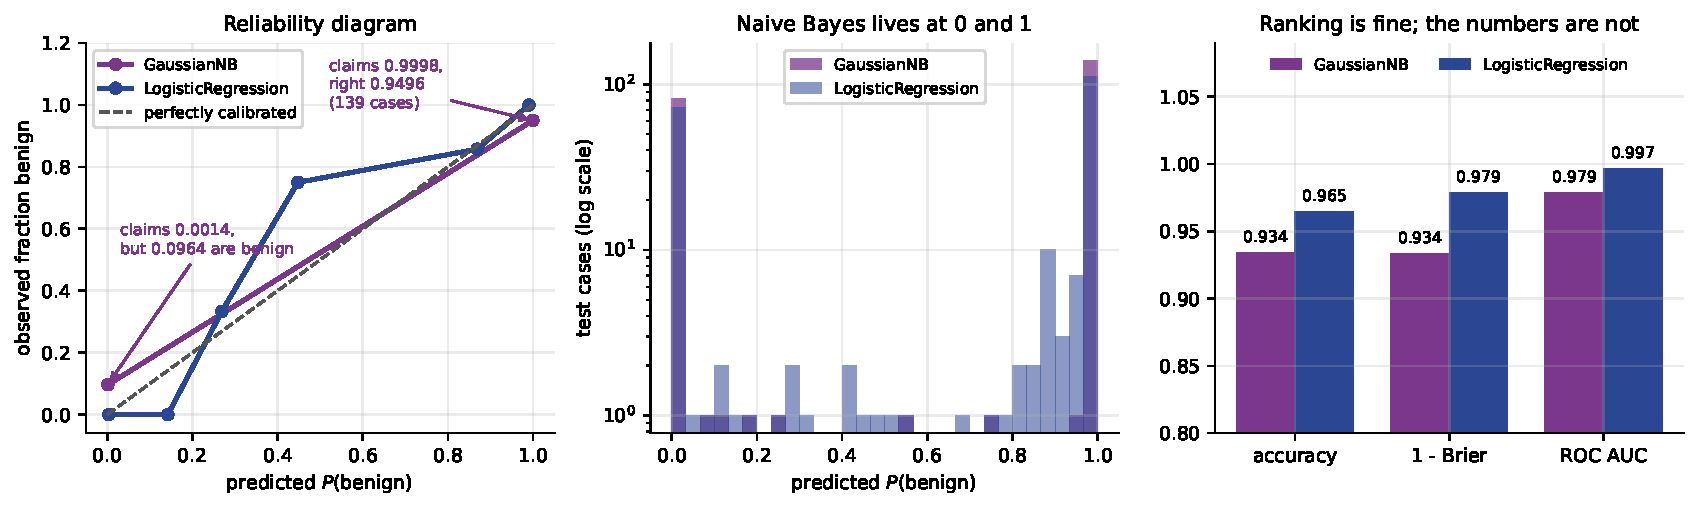
\includegraphics[width=0.92\textwidth]{calibration.pdf}
  \end{center}
  \begin{center}\small
    Left: the reliability diagram --- the purple curve should lie on the
    diagonal and does not. Centre: the histogram of predicted probabilities;
    naive Bayes has \emph{two} bars and almost nothing in between. Right: the
    same model scored three ways. \textbf{Its ROC AUC is $0.979$ --- the
    ranking is nearly as good as logistic regression's $0.997$ --- while its
    Brier score is three times worse.}
  \end{center}
\end{frame}

\begin{frame}[fragile,shrink=6]{Can it be repaired? Yes, afterwards}
\begin{outblk}
   model                               accuracy    Brier      AUC
   GaussianNB, raw                       0.9342   0.0663   0.9785
   GaussianNB + sigmoid                  0.9342   0.0626   0.9751
   GaussianNB + isotonic                 0.9211   0.0567   0.9646
\end{outblk}
\onslide<2->
\begin{columns}[T]
  \begin{column}{0.48\textwidth}
    \begin{block}{What calibration is}
      \footnotesize \texttt{CalibratedClassifierCV} fits a second, monotone
      model that maps the raw scores to honest probabilities --- a sigmoid
      (Platt scaling) or a step function (isotonic).
    \end{block}
  \end{column}
  \begin{column}{0.48\textwidth}
    \begin{alertblock}{Reported honestly}
      \footnotesize The Brier score improves both times, $0.0663$ to
      $0.0626$ and $0.0567$. The AUC does \emph{not}: the wrapper averages
      five fold-models each fitted on $80\%$ of only $341$ rows, and
      isotonic reorders ties. \textbf{Calibration repairs the numbers, and
      on a small sample it costs a little ranking.}
    \end{alertblock}
  \end{column}
\end{columns}
\begin{center}\small
  Practical rule: \textbf{use \texttt{predict} freely, treat
  \texttt{predict\_proba} with suspicion}, and calibrate before you use a
  naive Bayes probability to make a decision with a cost attached.
\end{center}
\end{frame}

% =====================================================================
\section[Where it hurts]{Where the independence assumption genuinely hurts}
\label{sec:hurts}

\begin{frame}[fragile,shrink=7]{Copy one feature and watch the accuracy fall}
Four genuinely independent informative features, classes separated by
$1.6$ standard deviations. Now add $k$ near-copies of feature $0$.
\begin{outblk}
    copies of f0    d  GaussianNB    LogReg  RandForest
               0    4      0.9475    0.9467      0.9367
               1    5      0.9350    0.9483      0.9350
               3    7      0.9083    0.9467      0.9283
               7   11      0.8633    0.9458      0.9267
              15   19      0.8367    0.9467      0.9233
              31   35      0.8200    0.9483      0.9133
   GaussianNB lost 0.1275 of accuracy; logistic regression lost -0.0017
\end{outblk}
\onslide<2->
\begin{outblk}
   and what it does to the confidence
      k= 0  mean confidence 0.9457   accuracy 0.9556   fraction > 0.999 0.2833   Brier 0.0331
      k=31  mean confidence 0.9916   accuracy 0.8139   fraction > 0.999 0.9139   Brier 0.1802
\end{outblk}
\onslide<3->
\begin{alertblock}{$0.9475 \rightarrow 0.8200$, on \emph{no new information}
--- and it gets \emph{more} certain}
  \footnotesize The added columns are copies: they contain nothing column $0$
  did not already contain. \textbf{Naive Bayes multiplies the same evidence
  thirty-two times}, because the product rule assumes each factor is a fresh
  observation. Logistic regression fits the columns jointly, splits the
  weight between them, and does not move at all. Meanwhile confidence rises
  $0.9457 \to \mathbf{0.9916}$ while accuracy falls
  $0.9556 \to \mathbf{0.8139}$. \textbf{That is the mechanism behind the
  previous section.}
\end{alertblock}
\end{frame}

\begin{frame}[fragile,shrink=7]{On real data: thirty columns that are ten
measurements}
\texttt{breast\_cancer} records ten cell measurements three ways each --- a
mean, a standard error and a ``worst'' value.
\begin{outblk}
   mean |correlation| between the 30 columns: 0.3949
   pairs with |r| > 0.9: 21 of 435
   feature set                          d  GaussianNB    LogReg
   all 30                              30      0.9385    0.9789
   the 10 'mean' columns               10      0.9104    0.9455
   the 10 'worst' columns              10      0.9456    0.9789
   mean + worst (20)                   20      0.9420    0.9789
\end{outblk}
\onslide<2->
\begin{center}\small
  \textbf{Ten columns beat thirty}: the \texttt{worst} block alone gives
  \texttt{GaussianNB} $0.9456$ against $0.9385$ for all thirty.
  \textbf{Dropping two-thirds of the data improved the model.}
\end{center}
\begin{alertblock}{}
  \centering\footnotesize
  So for naive Bayes, \textbf{de-duplicating correlated columns is a real
  modelling step}, not tidying. It is the one place where feature selection
  reliably pays for this algorithm.
\end{alertblock}
\end{frame}

\begin{frame}[fragile,shrink=8]{Drawn: counting the same evidence many times}
  \begin{center}
    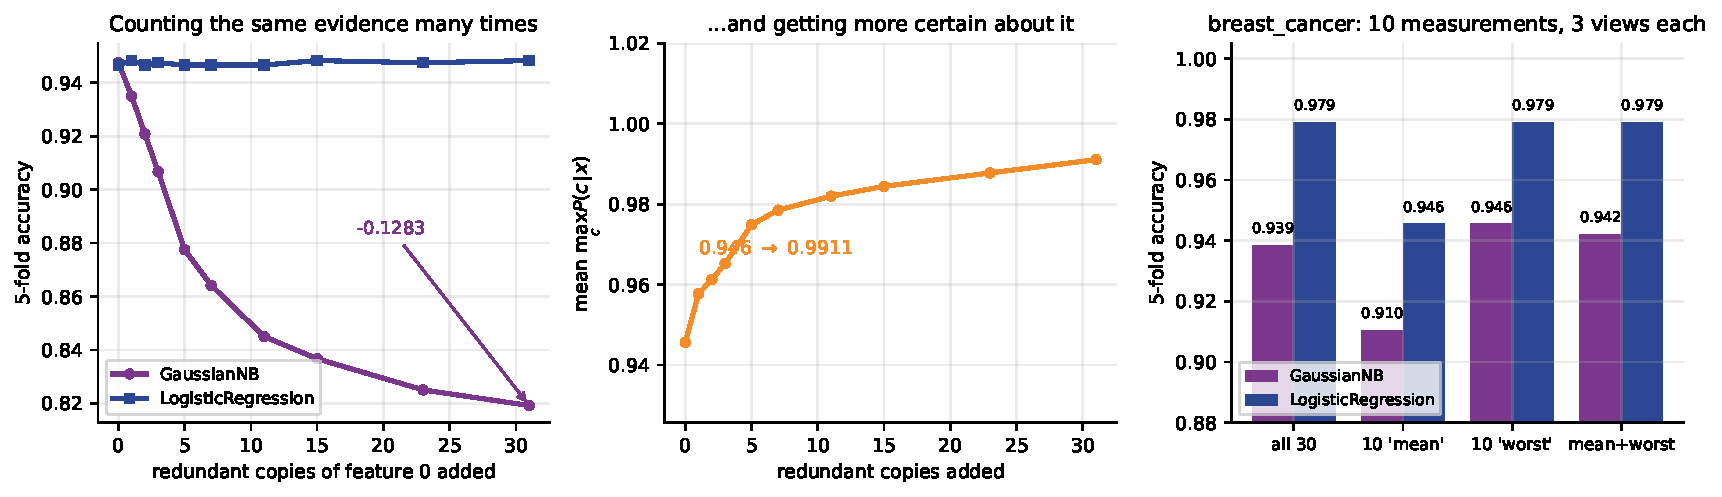
\includegraphics[width=0.92\textwidth]{correlated.pdf}
  \end{center}
  \begin{center}\small
    Left: accuracy against redundant copies --- purple falls, blue does not
    move. Centre: mean confidence over the same sweep, rising from $0.9457$ to
    $0.9911$ as accuracy falls. Right: the real \texttt{breast\_cancer}
    feature blocks.
  \end{center}
\end{frame}

\begin{frame}[fragile,shrink=7]{A different failure: XOR}
Two binary features, label $= u \oplus v$, plus a little noise. The four
$(u,v)$ cells hold $300$ rows each \emph{by construction}, so the symmetry is
exact and not a lucky sample.
\begin{outblk}
   GaussianNB   0.4600
   LogReg       0.4600
   RandForest   0.9833
      class 0: mean u 0.5063  mean v 0.4974  corr(u,v|y) +0.8621
      class 1: mean u 0.4819  mean v 0.4936  corr(u,v|y) -0.8573
\end{outblk}
\onslide<2->
\begin{alertblock}{Chance level, on a perfectly learnable problem}
  \footnotesize Read the last two lines. Within each class the means of $u$
  and $v$ are both about $0.5$: \textbf{each feature alone is completely
  uninformative}, so every per-feature factor $P(x_j \mid c)$ is identical
  for both classes and the product cannot distinguish them. All the signal
  lives in the \emph{correlation}, which is $+0.86$ in one class and $-0.86$
  in the other --- precisely what the naive assumption throws away.
\end{alertblock}
\onslide<3->
\begin{center}\small
  A random forest gets $0.9833$. \textbf{When the information is in the
  interaction, use a model that can represent interactions.}
\end{center}
\end{frame}

\begin{frame}[fragile,shrink=7]{So why does anyone still use it? Because of
this table}
Fit both models on a shrinking training set, average over $30$ random splits.
\begin{outblk}
    n train  GaussianNB    LogReg  RandForest
         20      0.9271    0.9276      0.9161
         40      0.9366    0.9502      0.9287
         80      0.9374    0.9640      0.9393
        200      0.9357    0.9711      0.9478
        400      0.9385    0.9763      0.9548
\end{outblk}
\onslide<2->
\begin{alertblock}{At $n = 20$ it is level with logistic regression}
  \footnotesize Twenty patients, thirty features. Naive Bayes estimates
  $30 \times 2$ means and $30 \times 2$ variances, each from ten rows, and
  scores $0.9271$. \textbf{It has almost no variance to bleed, because it
  never fits a joint anything.} By $n = 400$ logistic regression is four
  points ahead --- but you often do not have $400$ rows.
\end{alertblock}
\onslide<3->
\begin{center}\small
  Domingos and Pazzani's result, in a table: \textbf{a wrong probability
  model can still put the right class on top}, because the argmax only needs
  the ordering, not the values.
\end{center}
\end{frame}

% =====================================================================
\section{Summary}
\label{sec:summary}

\begin{frame}[shrink=18]{Summary --- fifteen lines}
  \begin{enumerate}\small
    \item Bayes' theorem is the product rule written twice and divided:
      $P(c \mid x) = P(x \mid c)P(c)/P(x)$. \textbf{Prior}, \textbf{likelihood},
      \textbf{evidence}, \textbf{posterior}. It is a rearrangement, not an
      assumption.
    \item The medical test: $1\%$ prevalence, $99\%$ sensitivity, $95\%$
      specificity. A positive result gives $P(D \mid +) = 99/594 =
      \mathbf{0.1667}$, not $0.99$. \textbf{The base-rate fallacy is
      confusing $P(D \mid +)$ with $P(+ \mid D)$.}
    \item In whole people: of $10{,}000$, $594$ test positive and $99$ are
      ill. \textbf{False positives outnumber true positives five to one.}
      Two million simulated people agree to $0.001$.
    \item Specificity, not sensitivity, is the lever: $95\% \to 99.9\%$ takes
      the posterior from $0.1667$ to $0.9091$. Raising prevalence to $20\%$
      takes it to $0.8319$.
    \item \textbf{ML} maximises $P(x \mid c)$, \textbf{MAP} maximises
      $P(x \mid c)P(c)$. On this evidence they disagree: ML says disease, MAP
      says no disease, because a likelihood ratio of $19.8$ cannot overcome
      prior odds of $99$.
    \item Posterior odds $=$ likelihood ratio $\times$ prior odds. One
      multiplication.
    \item The full joint likelihood needs $C(2^d-1)$ parameters: at $d=30$
      that is $2{,}147{,}483{,}646$ against $569$ training rows. It exceeds
      the data at $\mathbf{d = 9}$.
    \item \textbf{The naive assumption}: $P(x_1,\ldots,x_d \mid c) =
      \prod_j P(x_j \mid c)$ --- independence \emph{given the class}. On the
      tennis table it takes $70$ free parameters down to $\mathbf{12}$.
    \item By hand on $(\text{Sunny},\text{Cool},\text{High},\text{Strong})$:
      \emph{No} scores $0.02057143$, \emph{Yes} $0.00529101$, so
      $P(\text{No} \mid x) = \mathbf{0.795417}$ --- and
      \texttt{CategoricalNB} agrees to $7.68\times10^{-12}$.
    \item \textbf{Zero frequency}: $P(\text{Overcast} \mid \text{No}) = 0/5$
      makes the whole product $0$. Laplace, $(0+1)/(5+3) = 0.125$, turns
      $P(\text{No} \mid x)$ from $\mathbf{0.000000}$ into
      $\mathbf{0.278417}$. Twelve of the $36$ possible days contain a zero;
      on this table the \emph{label} never flips, but the posterior moves by
      up to $0.4356$.
    \item As $\alpha \to \infty$ the posterior tends to the prior $9/14 =
      0.6429$. $\alpha$ is a regularisation parameter: cross-validate it.
    \item \textbf{Logs.} A product of per-token probabilities hits exactly
      $0.0$ at $\mathbf{148}$ tokens. Multiplying instead of adding logs took
      test accuracy from $0.9722$ to $\mathbf{0.5056}$, silently. Recover a
      posterior with log-sum-exp: $a_{\max} + \log\sum e^{a - a_{\max}}$.
    \item \textbf{Gaussian NB} replaces counting with one mean and one
      variance per feature per class. Iris petal width $1.7$\,cm gives
      $P(\text{virginica}) = 0.685166$; boundaries at $0.6333$ and
      $1.6437$\,cm. Fits \texttt{digits} in \emph{one} pass against
      logistic regression's $32$ iterations.
    \item \textbf{Good classifier, bad probability estimator}: mean
      confidence $\mathbf{0.9936}$ against accuracy $\mathbf{0.9342}$; $93\%$
      of predictions above $0.999$; Brier three times worse than logistic
      regression while AUC is $0.979$ against $0.997$.
    \item \textbf{Correlated features are the mechanism.} Thirty-one copies
      of one column took accuracy $0.9475 \to 0.8200$ and confidence
      $0.9457 \to 0.9916$. On \texttt{breast\_cancer}, ten columns beat
      thirty. On XOR, naive Bayes scores $0.4600$. But at $n=20$ it ties
      logistic regression --- which is why it survives.
  \end{enumerate}
\end{frame}

\begin{frame}[shrink=3]{Before the next lecture}
  \begin{columns}[T]
    \begin{column}{0.48\textwidth}
      \begin{block}{Read}
        \texttt{notes.pdf} --- the full development, the derivation from the
        product rule, the complete smoothing treatment, and \textbf{10
        practice questions with worked solutions}.
      \end{block}
      \begin{block}{Do}
        Questions 1, 2, 3 and 5, \textbf{with a pen}. Question 1 is a
        base-rate calculation; question 3 is a full naive Bayes by hand with
        Laplace smoothing. These are the numerically examinable ones.
      \end{block}
    \end{column}
    \begin{column}{0.48\textwidth}
      \begin{exampleblock}{Next: ensemble methods}
        Bagging, boosting and random forests --- many weak models combined by
        vote. Carry one contrast across: \textbf{naive Bayes wins by making a
        strong wrong assumption and paying almost nothing for it; an ensemble
        wins by making no assumption and paying in computation.}
      \end{exampleblock}
      \begin{alertblock}{And a habit to start now}
        Any time you read a probability off a classifier, ask what it would
        take to check it. Bin the predictions, compare the claim with the
        outcome. \textbf{A model that is right $93\%$ of the time and says
        $99.4\%$ is lying to you politely.}
      \end{alertblock}
    \end{column}
  \end{columns}
  \begin{center}
    \small Materials: \texttt{\AMLRepoURL}
  \end{center}
  \slidesources{\AMLUnitVISources}
\end{frame}

\end{document}
